%----------------------------------------------------------------------------------------
%	PACKAGES AND OTHER DOCUMENT CONFIGURATIONS
%----------------------------------------------------------------------------------------

\documentclass[12pt]{scrartcl} % Font size

%----------------------------------------------------------------------------------------
%	PACKAGES AND OTHER DOCUMENT CONFIGURATIONS
%----------------------------------------------------------------------------------------

\usepackage{amsmath, amsfonts, amsthm} % Math packages

\usepackage{listings} % Code listings, with syntax highlighting

\usepackage[ngerman]{babel} % german language hyphenation

 \usepackage{setspace}

\usepackage[backend=biber, style=numeric-verb]{biblatex}
\addbibresource{literatur.bib}

\usepackage{graphicx} % Required for inserting images
\graphicspath{{Figures/}{./}} % Specifies where to look for included images (trailing slash required)

\usepackage{booktabs} % Required for better horizontal rules in tables

\numberwithin{equation}{section} % Number equations within sections (i.e. 1.1, 1.2, 2.1, 2.2 instead of 1, 2, 3, 4)
\numberwithin{figure}{section} % Number figures within sections (i.e. 1.1, 1.2, 2.1, 2.2 instead of 1, 2, 3, 4)
\numberwithin{table}{section} % Number tables within sections (i.e. 1.1, 1.2, 2.1, 2.2 instead of 1, 2, 3, 4)

\setlength\parindent{0pt} % Removes all indentation from paragraphs

\usepackage{enumitem} % Required for list customisation
\setlist{noitemsep} % No spacing between list items

%----------------------------------------------------------------------------------------
%	DOCUMENT MARGINS
%----------------------------------------------------------------------------------------

\usepackage{geometry} % Required for adjusting page dimensions and margins

\geometry{
	paper=a4paper, % Paper size, change to letterpaper for US letter size
	top=2.5cm, % Top margin
	bottom=3cm, % Bottom margin
	left=2.5cm, % Left margin
	right=2.5cm, % Right margin
	headheight=0.75cm, % Header height
	footskip=1.5cm, % Space from the bottom margin to the baseline of the footer
	headsep=0.75cm, % Space from the top margin to the baseline of the header
	%showframe, % Uncomment to show how the type block is set on the page
}

%----------------------------------------------------------------------------------------
%	FONTS
%----------------------------------------------------------------------------------------

\usepackage[utf8]{inputenc} % Required for inputting international characters
\usepackage[T1]{fontenc} % Use 8-bit encoding
\usepackage{textgreek}

\usepackage{mathptmx}
%\usepackage{fourier} % Use the Adobe Utopia font for the document

%----------------------------------------------------------------------------------------
%	SECTION TITLES
%----------------------------------------------------------------------------------------

\usepackage{sectsty} % Allows customising section commands

\sectionfont{\vspace{6pt}\centering\normalfont\scshape} % \section{} styling
\subsectionfont{\normalfont\bfseries} % \subsection{} styling
\subsubsectionfont{\normalfont\itshape} % \subsubsection{} styling
\paragraphfont{\normalfont\scshape} % \paragraph{} styling

%----------------------------------------------------------------------------------------
%	HEADERS AND FOOTERS
%----------------------------------------------------------------------------------------

\usepackage{scrlayer-scrpage} % Required for customising headers and footers

\ohead*{} % Right header
\ihead*{} % Left header
\chead*{} % Centre header

\ofoot*{} % Right footer
\ifoot*{} % Left footer
\cfoot*{\pagemark} % Centre footer
 % Include the file specifying the document structure and custom commands

%----------------------------------------------------------------------------------------
%	TITLE SECTION
%----------------------------------------------------------------------------------------

\title{	
	\normalfont\normalsize
	\vspace{200pt}
	\textsc{Valentin Heider Gymnasium}\\
	\vspace{10pt}
	\textsc{Jahrgang 2021/2023}\\
	\begin{figure}[h] % [h] forces the figure to be output where it is defined in the code (it suppresses floating)
	\centering
	
\includegraphics[width=0.5\columnwidth]{VHGLogo.jpg} 
	\end{figure}
	\vspace{25pt}\\
	
	\rule{\linewidth}{0.5pt}\\
	\vspace{20pt}
	{\huge Das SIR - Modell}\\
	\vspace{12pt}
	\rule{\linewidth}{2pt}\\
	\vspace{20pt}
	{\Large W Seminar Mathematik:}\\
	\vspace{12pt}\\
	{\Large Chaos, Fraktale und andere mathematische Faszinationen}\\
	\vspace{20pt}\\
	{\Large Herr Jan Neuendorf}\\
	\vspace{15pt}\\
}

\author{\LARGE Nicolas Martin}

\date{\normalsize 8.11.2022}

\begin{document}

\pagenumbering{Roman}
\maketitle % Print the title
\thispagestyle{empty}
\newpage

\doublespacing
\tableofcontents
\thispagestyle{empty}
\cleardoublepage
\onehalfspacing
\newpage

%----------------------------------------------------------------------------------------
\section{Einleitung}
\pagenumbering{arabic}

%GRENZWERTE DES GEBIETS, WEITERE BEKANNE EPIDEMIEN(rubella chickenpox influenza)

Das \textsl{Covid-19} Virus hat in den letzten Jahren Eindrucksvoll bewiesen, wie schnell sich eine Epidemie ausbreiten und zur Pandemie werden kann,  
Sowie welche verheerende Wirkung ebensolche auf die gesamte Bevölkerung und Wirtschaft der Welt haben. 
Immer wieder teilten Experten in den Medien neue Verhaltens- und Hygieneregelungen mit, durch welche die Verbreitung des Virus Verlangsamt werden konnte. Auch Prognosen über die Zukünftige Entwicklung der Pandemie wurden Veröffentlicht. 
Doch wie genau Berechnen Epidemiologen die Entwicklung einer Epidemie um Vorhersagen zu treffen und die geeignetsten Gegenmaßnamen zur Eindämmung einer solchen zu ermitteln?\\
\\
Diese Literaturarbeit soll zunächst das \textbf{SIR-Modell} mit allen Voraussetzungen Betrachten, Die Einhergehenden Differenzialgleichungen und die Basisreproduktionszahl Mathematisch Analysieren und unter Betrachtung der Flexibilität des Modells evaluieren. 
Des weiteren veranschaulicht die Arbeit das Mathematische Chaos des Modells 
ferner welche Veränderungen mit verschiedenen Abwandlungen der Formeln und Variablen Einhergehen. 
Die Präzision und Effektivität in der Anwendung soll durch Den Fall \textsl{Covid-19} verdeutlicht und mit der Jährlichen Influenza-Grippe verglichen werden. 
Ausgenommen Der Fallbeispiele und der Dynamischen Gesamtbevölkerung werden keine Abweichungen des Modells im Detail Besprochen. 

%----------------------------------------------------------------------------------------

\newpage
\section{Grundlagen Des SIR-Modells}

Wenn man den Verlauf einer Epidemie von Anfang bis Ende anhand eines Mathematischen Modells beschreiben möchte, ist das \textbf{SIR-Modell} mit nur zwei Parametern und drei Differentialgleichungen in der einfachsten Form ideal, um sich einen groben Überblick zu verschaffen \cite{4}.
Im diesem Kapitel wird auf den Hintergrund, die Optionen und Limitierungen und die damit Einhergehenden Möglichkeiten der Anwendung des Modells eingegangen.

%------------------------------------------------

\subsection{Entstehungsgeschichte}

Das \textbf{Kermack-McKendrick Modell} ist die Bekannteste Ausführung des \textbf{SIR-Modells} welches von den Infektionsepidemiologen \textsl{William Ogilvy Kermack} und \textsl{Anderson Gray McKendrick} im Jahr 1927 Im Zusammenhang mit dem Artikel 
\textsl{"'A contribution to the mathematical theory of epidemics"'} \cite{7} im Auftrag der \textsl{"'Royal Society London"'}Entwickelt und Veröffentlicht wurde \cite{6}.\\

\textsl{"'The paper became a classic in infectious disease epidemiology and has been cited innumerable times"'} \cite{6} \\

%In besagtem schreiben wurde eine These von W.H. Hamer bewiesen, welche statuiert das eine Epidemie nicht erst dann vorbei ist wenn alle %suszeptiblen personen Einmal infiziert wurden sondern durch eine \textsl{"'... auf Anzahlen und Dichten basierenden mathematischen %Übertragungstheorie"'} \cite[s. 81]{2} bestimmt wird. \cite{2}
Seit dem wird das \textbf{SIR-Modell} und Variationen Weltweit verwendet um den Verlauf verschiedenster Infektionen
wie Beispielsweise Ebola, Masern und Influenza nachzuvollziehen und/oder Vorherzusagen. \cite{3}

%Ross ?

%------------------------------------------------

\subsection{Voraussetzungen}

Da das \textbf{SIR Modell} als relativ simpel gilt, kommt es mit einigen Voraussetzungen die erfüllt werden müssen damit es Anwendbar ist.
Zuerst Muss die Gesamtbevölkerung \textit{N} in drei Kategorien unterteilt werden:

\begin{itemize}
	\item \textit{S}: Suszeptibel (engl. Susceptible)
	\item \textit{I}: Infiziert (engl. Infected)
	\item \textit{R}: Entfernt (engl. Removed)
\end{itemize}
\normalsize

Wobei (\textit{S}) alle Infizierbaren Individuen, (\textit{I}) alle Infizierten und \textbf{gleichzeitig} Infektiösen und (\textit{R}) alle Genesenen oder verstorbenen beinhaltet.  Zu beachten ist das sich Individuen jeweils immer nur in Einer Population befinden können und sich Individuen der Population 
(\textit{R}) kein weiteres mal Infizieren können da sie als Immun Gelten. Hierbei ist es Egal ob das Individuum Genesen oder Verstorben ist (vgl. Abb. 2.1) \cite{4}.
Alle Populationen Interagieren untereinander mit der selben Wahrscheinlichkeit die von nur zwei Parametern beta (\textbeta) und gamma (\textgamma) Beeinflusst wird. 
\textbeta \space steht hier für die Übertragungsrate (engl. transmission rate) welche angibt, wie schnell Individuen der Suszeptiblen Population in die Infizierte Population übergehen. 
\textgamma \space hingegen stellt hier die Erholungsrate (engl. recovery rate) dar, und gibt an wie schnell die Population \textit{I} sich erholt oder verstirbt.
Es wird davon ausgegangen das \textit{N}, \textbeta, \textgamma \space \textbf{Konstant} und \textbf{Positiv} sind sind.
Zu Beginn der Epidemie sei die Menge der Population \textsl{R} gleich Null, die Menge \textsl{S} ungefähr \textit{N} und die Menge \textit{I} ungefähr Null (Mindestens ein Individuum Infiziert), dar das \textbf{SIR-Modell} von einer neuen Infektion ausgeht, zu welcher am Anfang keine Immunität existiert.

	\begin{figure}[h]
	\centering
	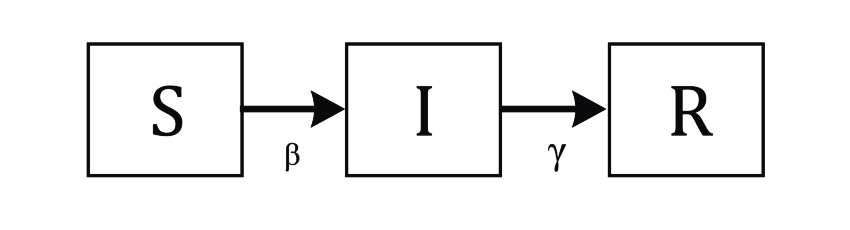
\includegraphics[width=0.8\columnwidth]{SIR-model-flowchart.png} 
	\caption[SIR Gruppenverteilung,\newline https://www.researchgate.net/figure/SIR-model-flowchart\textunderscore fig8\textunderscore 318394911]{SIR Gruppenverteilung}
	\end{figure}

%------------------------------------------------

\subsection{Anwendung}

Das \textbf{SIR-Modell} in der hier dargestellten Form kann das verhalten einer Epidemie anhand zwei unveränderlicher Parameter Darstellen und zeigt so auf wie lange es braucht, bis eine Bevölkerungsgruppe die Infektion überstanden hat. Auch die menge an Personen, welche bis zum Ende in der Suszeptiblen Gruppe (\textit{S}) verblieben sind kann ermittelt werden. 
Eine große Limitierung des Modells findet sich in der Tatsache, das es durch den Einfachen Aufbau mit wenigen Parametern und Unrealistischen Voraussetzungen wie einer konstanten Bevölkerung oder der direkten Infektiösität von Individuen nur einen Ungefähren verlauf, jedoch keine präzise noch detaillierte Auskunft über Realszenarien bietet.
Durch die Annahme das zu beginn keine Immunität existiert, und die Parameter als konstant betrachtet werden ist das Modell des weiteren nicht zur Berechnung von Infektionswellen geeignet.
Allerdings bildet das \textbf{SIR-Modell} eine Grundlage für komplexere Modelle, welche für bestimmte Infektionen und Umstände angepasst werden, und somit detailreiche Prognosen sowie Berichte über Die Entwicklung Bereitstellen können.
So wird beispielsweise in \textsl{"The SIR Model with Vital Dynamics"} \cite{5} durch hinzufügen von Parametern für Geburten und Tode die Gesamtbevölkerung als Dynamisch Betrachtet, was bereits näher an ein Realbeispiel herankommt.
Dieses Modell wird in \textsl{3.3} Genauer Beschrieben.\\
Zusätzlich können die Gruppen erweitert oder entfernt werden, was dann zu Modellen wie dem 
\textbf{SIRS-Modell}, welches eine erneute Infektion ermöglicht und somit auch für Infektionswellen genutzt werden kann, dem \textbf{SEIR-Modell}, welches eine Personengruppe hinzufügt die Infiziert wurde, jedoch noch nicht ansteckend ist(\textit{E}: Exposed) oder dem \textbf{SI-Modell}, in welchem Individuen keine Immunität aufbauen, führen kann.
Eine weiterer Anwendungsgrund des Modells ist die Bestimmung der Basisreproduktionszahl (siehe \textsl{3.2}), welche angibt, ob sich eine Infektion zu einer Epidemie entwickelt, sich Endemisch hält oder auf Dauer ausstirbt \cite{2}.
So ist das Modell als solches zwar nur als ein Mathematisches Idealverhältnis einer Epidemie von nutzen, doch ist es ein Essenzieller teil der Modernen Infektionsepidemiologie welches von Forschen auf der Ganzen Welt dafür genutzt wird, Virale Krankheiten zu dokumentieren und den Ausbruch in eine Epidemie zu verhindern \cite{3}.
%----------------------------------------------------------------------------------------

\section{Mathematischer Aufbau}

Nachdem die Wichtigsten Begriffe und Bedingungen für das \textbf{SIR-Modell} nun bekannt sind Widmet sich dieses Kapitel der Funktion und Zusammensetzung des Modells auf mathematischer Ebene, woraufhin der Fokus auf die Basisreproduktionszahl sowie auf einige Abweichungen des Modells gelegt wird, bis schlussendlich die Chaotischen Züge des Modells analysiert werden.
Wenn eine konstante Bevölkerung \textit{N} in drei Gruppen aufgeteilt wird kann \textit{N} jetzt zu jedem Zeitpunkt (\textit{t}) folgendermaßen definiert werden \cite{3,4}:

$$ \large\textit{S}_{(t)} + \textit{I}_{(t)} + \textit{R}_{(t)} = \textit{N}\normalsize $$

Oder Proportional:

$$ \large\textit{S} + \textit{I} + \textit{R} = 1 $$
\begin{center}
Wobei gilt: \textit{S} > 0, \textit{I} > 0, \textit{R} \geq 0.
\end{center}

Während die Modell definierenden Parameter \textbeta\space und \textgamma\space konstant sind, Verändern sich die Größen \textit{S}, \textit{I} und \textit{R} im verlauf von \textit{t}. Man spricht von einem Geschlossenen System \cite{4}.

%------------------------------------------------

\subsection{Variablen des SIR Modells}

Zunächst werden die Konstanten Parameter noch einmal genauer betrachtet: Die Erholungsrate \textgamma\space Beeinflusst, wie lange die Infektion durchschnittlich anhält und wird folgendermaßen berechnet:

$$ \gamma = \frac{1}{T} $$
\\

Wenn also \textit{T} drei Tagen entspricht, ist \textgamma\space ein Drittel. Die Übertragungsrate \textbeta\space hingegen beschreibt, wie oft eine Begegnung der Gruppen \textit{S} und \textit{I} vorkommt, welche zu einer Infektion des Individuums der \textit{S} Population führt \cite{2}. 
Im Klassischen \textbf{SIR-Modell} wird von einer vollkommen Zufälligkeit der Kontakte ausgegangen, der Parameter kann durch weitere Faktoren wie Hygiene erweitert werden \cite{2,7}.\\
Da das Modell die Veränderung nur In eine Richtung zulässt (\textit{S} \textrightarrow\space \textit{I} \textrightarrow\space \textit{R}) lässt sich feststellen das die menge \textit{S} nur Abnehmen, und die menge \textit{R} nur zunehmen kann, und beide von \textit{I} beeinflusst werden.
Anhand dieser Informationen lassen sich folgende nichtlineare Differenzialgleichungen für die Änderungsraten, also die Populationsgrößen Veränderung, zu dem Zeitpunkt \textit{t} aufstellen:

$$ \frac{\Delta S}{\Delta t} = -\beta\space S I $$
\begin{center}
\textsl{Änderungsrate der Suszeptiblen Population s'(\textit{t})}
\end{center}

Die Suszeptible und die Infizierte Population haben den Parameter \textbeta \space gemeinsam. \textit{S} wird mit der rate \textbeta \space eine Menge an Individuen abgezogen (-\textbeta) und dann \textit{I} hinzugefügt. Da \textit{I} aus mehreren Infizierten Individuen besteht, welche jeweils \textbeta\space viele Suszeptible anstecken können, wird \textbeta\textit{S} mit \textit{I} multipliziert.
Die Population der Entfernten Individuen wird berechnet indem der Parameter \textgamma\space mit \textit{I} mal-genommen wird, da \textit{I} mit der rate \textgamma\space Entfernt wird \cite{7,3}:

$$ \frac{\Delta R}{\Delta t} = \gamma I $$
\begin{center}
\textsl{Änderungsrate der Entfernten Population r'(\textit{t})}
\end{center}


Da alle Gleichungen zu jedem Zeitpunkt zusammen 1 Ergeben müssen (\textit{S} + \textit{I} + \textit{R} = 1) und \textit{I} ein Faktor der anderen Gleichungen ist, kann s'(\textit{t}) durch Kombination der anderen Gleichung und Umkehrung der Parameter bestimmt werden
 \cite{3, 4}:

$$ \frac{\Delta I}{\Delta t} = \beta\space S I - \gamma I $$
\begin{center}
\textsl{Änderungsrate der Infizierten Population s'(\textit{t})}
\end{center}

Hier bekommt \textit{I} Zuwachs von \textit{S} mit dem Parameter \textbeta\space und nimmt mit dem Parameter \textgamma\space ab.

%------------------------------------------------

\subsection{Reproduktionsrate einer Infektion}

Wenn eine aktuelle Infektion mit dem \textbf{SIR-Modell} Betrachtet wird, soll an erster stelle erkenntlich gemacht wie sich die Infektion Verhält oder Verhalten wird. Es gibt Drei Verhaltensweisen, die durch das \textbf{SIR-Modell} festgestellt werden können: Endemisch wird eine Infektion benannt, welche regelmäßig an einem Ort auftritt und einigermaßen Konstante Infektionen aufweist. Epidemisch wird eine Infektion dann genannt, wenn sie an einem Ort unregelmäßig auftritt und schneller Neuinfektionen auftreten wie bereits Infizierte Genesen/Sterben, sich also Verbreitet. Eine globale Epidemie wird als Pandemie bezeichnet und nicht separat von dem \textbf{SIR-Modell} erfasst. Das Epidemisch Verhalten wird in zwei Phasen aufgeteilt: die Ausbreitung und den Rückgang der Epidemischen Phase. Das kommt daher das nach einer gewissen zeit die Meißen oder alle Individuen In die Infizierte oder Entfernte Population aufgerückt sind, sodass Neuinfektionen nicht mehr oder nur schwer möglich sind, sodass die Infektionswelle abflacht \cite{3,5}. Das \textbf{SIR-Modell} ermöglicht die Berechnung der sogenannten Basisreproduktionszahl  $r_{0}$
welche zu beginn der Infektion t = 0 das zukünftige Verhalten der Infektion angibt. Berechnet wird diese anhand der beiden Parameter \textbeta\ und \textgamma\space da diese ja die zu und Abnahme der Population \textit{I} beschreiben. Des weiteren spielt auch die proportionale Größe von \textit{S} eine rolle, da zur Infektion ein Suszeptibles Individuum benötigt wird. Da zu beginn des Modells \textit{S} ungefähr 1 ist, kann dieser Faktor zur Berechnung der Basisreproduktionszahl Vernachlässigt werden. Deshalb gilt Solange die Übertragungsrate \textbeta\space größer als die Erholungsrate \textgamma\space ist nimmt die menge der Population \textit{I} zu. Die Rechnung dazu sieht folgendermaßen aus \cite{6,3}:

$$ r_{0} = \frac{\beta}{\gamma} $$

\begin{center}
\textit{r_{0} > 1 =} \textnormal{Epidemisch}, r_{0} \approx 1 = \textnormal{Endemisch}, r_{0} < 1 = \textnormal{Rückgängig.}
\end{center}
Im Fall von R = 2 Infiziert Jedes Individuum der Population \textit{I} Zwei weitere Personen, bevor es In \textit{R} übergeht. In diesem Fall wird von Exponentiellem Wachstum gesprochen.
Wenn man die derzeitige Reproduktionszahl eines Zeitpunkts \textit{t} ermitteln möchte, um herauszufinden in welchem zustand sich die Infektion befindet, muss die Änderungsrate von \textit{S} berücksichtigt werden:

$$ r_{t} = \frac{\beta S_{t}}{\gamma} $$

Mithilfe dieser Gleichung lässt sich beispielsweise erkennen, welchen Effekt getroffene Maßnahmen (Social Distancing, Impfung) auf die Ausbreitung der Infektion haben.

%------------------------------------------------

\subsection{Graphische Darstellung Des SIR-Modells}

Ein Essenzieller Part des \textbf{SIR-Modells} ist die Graphische Darstellung des Infektionsverlaufs um eine visuelle Übersicht der Epidemie für die Allgemeinheit, und das schnelle auslesen von Daten an spezifischen Punkten zu haben.
In einem Koordinatensystem stellt die x-Achse die Zeit in Tagen, und die y-Achse die Bevölkerungsanzahl dar. Drei Graphen der in 3.1 angesprochenen Differenzialgleichungen zeigen die Änderung der Größe der jeweiligen Population auf.
Auch hier gilt das zu jedem Zeitpunkt die Summe der Flächen die Größe \textit{N} ergibt welche so eine Horizontale Asymptote für die Graphen bildet (Abb. 3.1).
Die Startwerte der Gruppen an t = 0 sind: 
$S_{0} \approx 1, I_{0} \approx 0$ wobei: $ S_{0} < 1, I_{0} > 0$ sodass beide zusammen die menge 1 Ergeben \cite{4}.
Da zu beginn kein Individuum Immunität besitzt und sich mindestens eine Infizierte Person in der Bevölkerung befinden muss, um den Ausbruch Auszulösen. Daher gilt: $R_{0} = 0, R_{0} \geq 0 $(nicht zu verwechseln mit der Basisreproduktionszahl $r_{0}$).
Anhand dieser Grafik lässt sich auslesen wann das Wachstum der Epidemie endet, wann sie ausstirbt sowie die menge der Individuen die zu keinem Zeitpunkt infiziert waren \cite{1}.

	\begin{figure}[h]
	\centering
	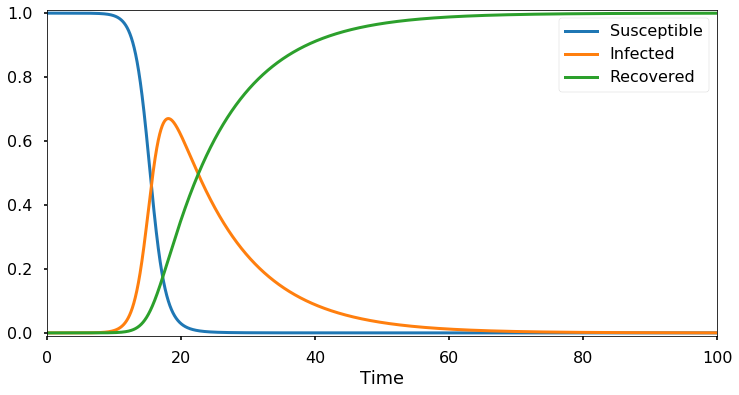
\includegraphics[width=0.8\columnwidth]{SIR-model-graph.png}
	\caption[SIR Infektionsverlauf,\newline https://www.davidketcheson.info/2020/03/17/SIR\textunderscore model.html]{SIR Infektionsverlauf}
	\end{figure}

%------------------------------------------------

\subsection{Variationen des SIR-Modells}

Nachdem die Grundlegenden Rechnungen und Parameter des \textbf{SIR-Modells} nun bekannt sind, werden im folgenden einige gängige Variationen des Modells genauer betrachtet. Wie bereits Erwähnt ist das Modell prädestiniert dafür, verändert oder erweitert zu werden um akkuratere Berechnungen zu Epidemien zu ermöglichen. Diese Veränderungen können das hinzufügen weiterer Populationen, Parameter, sowie das anpassen der Startbedingungen beinhalten \cite{5}.

%---------------------

\subsubsection{Modell zur Berechnung von Infektionswellen}

Wie am Beispiel \textsl{Covid-19} zu erkennen ist, gibt es Epidemien die keine oder nur Temporäre Immunität erlauben, was bedeutet, das Infektionswellen entstehen in welchen die Infektion ausbricht und wieder zurückgeht. Um das \textbf{SIR-Modell} für eine solche Situation anzupassen, kann Entweder die Entfernte Gruppe durch eine Suszeptible ersetzt werden was \textbf{SIS-Modell} genannt wird, oder eine weitere Suszeptible Gruppe zu einem \textbf{SIRS-Modell} angefügt werden. Die Startbedingungen und Parameter für das \textbf{SIS-Modell} bleiben dieselben des \textbf{SIR-Modells}. Aus den Drei Differentialgleichungen werden zwei:

$$ \frac{\Delta S}{\Delta t} = -\beta\space S I + \gamma I $$
$$ \frac{\Delta I}{\Delta t} = \beta\space S I - \gamma I$$

\textit{S} nimmt mit der Infektionsrate \textbeta\space ab, bekommt jedoch die menge der Erholungsrate \textgamma\space dazu, während für \textit{I} das genaue Gegenteil gilt. Individuen bewegen sich so von \textit{S} zu \textit{I} in einem Ewigen Kreislauf
 \cite{5}. Das \textbf{SIRS-Modell} wird eingesetzt, wenn eine nur temporäre Immunität besteht, wie es bei \textsl{Covid-19} der Fall ist. Diese Variation des Modells führt den Parameter \textepsilon\space als durchschnittliche Immunitätsdauer ein. Hier werden die Änderungsraten angepasst indem Individuen von \textit{R} mit der rate \textepsilon\space zu \textit{S} übergehen, was erneut in einem Kreislaufmodell Endet \cite{8}:

$$ \frac{\Delta S}{\Delta t} = -\beta\space S I + \epsilon R $$
$$ \frac{\Delta I}{\Delta t} = \beta\space S I + -\gamma I $$
$$ \frac{\Delta T}{\Delta t} = \gamma I - \epsilon R $$

%---------------------

\subsubsection{Modell mit dynamischer Gesamtbevölkerung}

In der Realität gibt es eine menge Faktoren, welche die Bevölkerung nicht Konstant halten. Das \textbf{SIR-Modell} mit \textbf{Dynamischer Bevölkerung} versucht durch die erweiterten Parameter \textnu\space für Geburten und \textmu\space für Todesfälle einige der wichtigsten Faktoren einer dynamischen Bevölkerung miteinzubeziehen. Neugeburten werden in die Suszeptible Population eingeordnet, während Tode in jeder Population Präsent sind. Dementsprechend werden diese Parameter zu den Änderungsraten hinzugefügt oder abgezogen \cite{8}:

$$ \frac{\Delta S}{\Delta t} = -\beta\space S I + \nu - \mu S $$
$$ \frac{\Delta I}{\Delta t} = \beta\space S I - \mu I $$
$$ \frac{\Delta R}{\Delta t} = -\beta\space S I - \mu R $$

%------------------------------------------------

\section{Mathematisches Chaos des SIR-Modells}

leicht veränderte startwerte, starke abweichung (100% social d vs. 90% social d)

\newpage
\subsection{Einflussfaktoren}

impfung, distancing, Hygiene, Mutationen

%----------------------------------------------------------------------------------------

\newpage
\section{Fallbeispiele}

epic Explanation

%------------------------------------------------

\subsection{Covid 19}

%------------------------------------------------
\newpage
\subsection{Jährliche flu}

%----------------------------------------------------------------------------------------
\newpage
\section{Fazit}

%----------------------------------------------------------------------------------------

\newpage
\setlength{\bibitemsep}{\baselineskip}
\printbibliography[heading=bibintoc]
\thispagestyle{empty}
\listoffigures

\end{document}
